\documentclass[letterpaper]{aamas2010}
%\usepackage{ijcai09}
\usepackage{amssymb}
%\usepackage[english]{babel}
\usepackage{latexsym}
\usepackage{amsfonts}
\usepackage{amsmath}
\usepackage{graphicx}
\usepackage{algorithmic}
%\usepackage{times}
\usepackage{subfigure}
%\usepackage{natbib}
%
\def\sharedaffiliation{%
\end{tabular}
\begin{tabular}{c}}
%

\newtheorem{assume}{{\bf Assumption}}

\numberofauthors{4} 


%\author{\alignauthor Zinovi Rabinovich$^{\dagger}$\\
%  \email{zr@ecs.soton.ac.uk}
%\alignauthor Lachlan Dufton$^*$\\ 
%  \email{ltdufton@cs.uwaterloo.ca}
%\alignauthor Kate Larson$^*$\\
%  \email{klarson@cs.uwaterloo.ca}
%\and
%\alignauthor Nicholas R. Jennings$^{\dagger}$\\
%  \email{nrj@ecs.soton.ac.uk}
%\sharedaffiliation
%  \affaddr{$^{\dagger}$Electronics and Computer Science, University of Southampton, United Kingdom}\\
%  \affaddr{$^*$Cheriton School of Computer Science, University of Waterloo, Canada}\\
%} 

%\alignauthor Zinovi Rabinovich\\
%\alignauthor Lachlan Dufton\\ 
%\alignauthor Kate Larson\\
%\alignauthor Nicholas R. Jennings
%}

\title{Policy  Teaching by a Modulation of the Transition Model}

\begin{document}

\maketitle

\begin{abstract}
There are three main teaching techniques applied by people: by
demonstration, by incentive, by environment dynamics
modification. While the first two have been mapped into intelligent
agent models, to the best of our knowledge, the third one has yet to
be instantiated.  Teaching by demonstration has found a significant
expression in robotics, while teaching by incentive has been
researched from the game theoretic perspective, where an interested
party attempts to manipulate other players by modifying their payoff
function.

In this paper we explicitly focus on the the implications of allowing
the interested party (teacher, in our model) to modify the
\emph{dynamics} of the environment, while leaving the reward function
of the agent alone. We first introduce a way to measure the divergence
between the realised and the passive (when no modification is applied
by the teacher) environment developments in a Markovian system. This
measure naturally incorporates and balances the teacher's effort and
the deviation of the learner's performance from an ideal reference,
that which the teacher is interested in. It also allows us to
formulate the teacher's problem as a planning and control problem, and
solve it using classical analytical and numerical tools.
\end{abstract}

\section{Introduction}
%\nocite{fleming_hernandez-hernandez_CDC_97}
%\nocite{todorov_2009_framework_sup}
%\nocite{todorov_2009_framework}
%\nocite{ng_russell_2000}
%\nocite{zhang_parkes_2009_ed}
%\nocite{dufton_larson_2009}

There are three main teaching techniques applied by people: by
demonstration, by incentive, by environment dynamics
modification. While the
first two have been mapped into intelligent agent models, to the best
of our knowledge, the third one has yet to be instantiated.

Teaching by demonstration has found a significant expression in
robotics~\cite{argal_etal_2009}. However, these mostly assume that the
learner actually wishes to learn the task, as well as a certain
benevolence on behalf of the teacher with respect to the learned
task.

On the other hand, teaching by incentive has been formalised in a way
that allows to the teacher to have an interest that may contradict
that of the learner. In more detail, recently, Zhang \emph{et al}
introduced a general framework for \emph{environment
  design}~\cite{Zhang09:General}. In environment design an interested
party attempts to influence the behaviour of an agent by making limited
changes to the agent's environment. Although in general this may
include environment dynamics modification, Zhang \emph{et al} have
concentrated on teaching by incentive. In particular, Zhang \emph{et
  al} have allowed their interested party to modify the cost function
of an agent in a linear programming example~\cite{Zhang09:General}, or
to modify the rewards of an agent acting in an environment modelled as
an MDP~\cite{zhang_parkes_2008,Zhang09:Policy}.

In this paper we explicitly focus on the the implications of allowing
the interested party (teacher, in our model) to modify the
\emph{dynamics} of the environment, while leaving the reward function
of the agent alone. We first introduce a way to measure the divergence
between the realised and the passive (when no modification is applied
by the teacher) environment developments in a Markovian system. This
measure naturally incorporates and balances the teacher's effort and
the deviation of the learner's performance from an ideal reference,
that which the teacher is interested in. It also allows us to
formulate the teacher's problem as a planning and control problem, and
solve it using classical analytical and numerical tools.


While our model may be cast as an example of environment design, we
note that our instantiation differs significantly from the particular
cases studied by Zhang \emph{et al}, and therefore creates a separate
line of study. In fact, representing the teacher's task as a control
problem is far more reminiscent of the work by Banerjee and
Peng~\cite{banerjee_peng_2005}, although it too focuses on the reward
modification.

To realise the necessity and importance of teaching by
environment dynamics modification consider the following real life
scenario. A parent wishes to teach a child to ride a bicycle. The
parent may {\em demonstrate} by riding the bicycle. However, in
practice, this does not yield good results when the child attempt to
repeat the task. It is also possible to promise an {\em incentive}, be
that a candy or a trip to the movies. Unfortunately, although
increasing the child's efforts, this does not facilitate the learning
process. The most practical thing to do in this case, is to {\em
  modify the dynamics} -- add safety wheels to the bicycle. Gradually
raising the safety wheels, allows the child to accustom to the
complete range of motion possibilities and, eventually, ride an
unabridged bicycle version.

In what follows we will formally define teaching by dynamics
modification given a learning algorithm we wish to teach
(Section~\ref{sec: GeneralModel}). We will also provide a specialised
version of the formalism for a specific MDP solution technique --
Policy Iteration (PI) algorithm (Section~\ref{sec: TOP-PI}). $\{\{$
Our experiments in Section~\ref{sec: experiments} will compare the
performance of PI with and without dynamics modification. $\}\}$. We
will then conclude in Section~\ref{sec: future work} with a discussion
of further development teaching by dynamics modification.


%%%%%%%%%%%%%%%%%%%%%%%%%%%%%%
\section{Interaction Model}\label{sec: GeneralModel}
%%%%%%%%%%%%%%%%%%%%%%%%%%%%%%

In this section we provide a high level description of the problem and
general framework.  In the next section we provide a particular
instantiation of our framework.

Our framework consists of a stochastic environment and two agents, a
\emph{learner} and a \emph{teacher}.  The learner acts within the
environment, taking actions and receiving feedback in the form of
rewards, which depend on the action taken and the current state of the
environment in which the agent finds itself.  We assume that the
learner is rational and thus attempts to find a \emph{policy} which
describes what action to take in each environment state, so as to
maximises its expected reward.  The teacher, on the other hand, does
not act \emph{in} the environment, but rather acts \emph{on} the
environment.  In particular, the teacher has some desired
\emph{reference policy}, $\pi^*$, that it wishes the learner to
follow, but is unable to force the agent to take any particular
action.  Instead, it is able to modify the environment's
\emph{dynamics} in order to influence the policy choice of the
learner. That is, the teacher's actions are able to influence the way
the environment state changes in response to the learner's actions,
and thus influence the policy of the learner. Dynamics modifications
come at a cost, however, and thus the goal of the teacher is to
minimise the modifications it must make to the environment dynamics
while at the same time ensuring that the policy followed by the
learner is close enough to the desired reference policy.

We model the problem by $\langle S, A, c,\gamma, U,T\rangle$ where:
\begin{itemize}
\item $S$ is the set of states, 
\item $A$ is the set of actions available to the learner,
\item  $c:S\times A\times S\rightarrow\mathbf{R}$ is the reward (or
  cost) function of the learner. $c(s',a,s)$ is the reward received by
  the learner if it has applied action $a\in A$ and the environment
  moved from state $s\in S$ to state $s'\in S$,
\item $\gamma \in (0,1)$ is a discount factor,   

\item $U$ is the set of actions (modifications to the environment)
  that the teacher can apply and $u_t\in U$ is the modification made
  at time $t$,

\item $T:S\times A\times U\rightarrow\Delta(S)$ describes the
  environment dynamics where $T_u(s'|s,a)\equiv T(s'|s,a,u)$ is the
  probability that the state will change from $s$ to $s'$ if the
  learner has applied action $a\in A$ and the teacher chose
  environment modification $u\in U$.

%Denote $T_{u_t}(s'|s,a)=T(s'|s,a,u_t)$. 
 
 %% KATE NEEDS TO THINK ABOUT THE NEXT BIT SINCE SHE DOES NOT LIKE THE 
 %% NOTATION.
 %% KATE HAS THOUGHT ABOUT IT AND STILL DOES NOT LIKE THIS NOTATION. 
 %% SUGGESTIONS ARE NOT IN THE TEXT.
We assume that there exist a null
  modification $u^*\in U$, so that $T^*=T_{u^*}$ are the nominal,
  passive dynamics of the environment.
  
  [KATE: I DO NOT LIKE THE NOTATION USED ABOVE SINCE WE USE * FOR TWO THINGS;  
  DESIRED POLICY OF THE TEACHER AND THE UNCHANGED ENVIRONMENTS. TOO  
  CONFUSING.
  INSTEAD, I PROPOSE THAT WE USE $u^0\in U$ TO REPRESENT THE NULL MODIFICATION 
   $T^0=T_{u^0}$.  I HAVE NOT MADE ANY OF THESE CHANGES IN THE TEXT.]
\end{itemize}


While applying its iterative policy calculation algorithm, the learner
faces a sequence of Markov Decision Problems (MDPs)~\cite{puterman_book_94},
 given by tuples $<S,A,U,T_{u_t},R>$, although it is not aware of the dynamics
modulation and proceeds as if they were homogeneous. 
\begin{assume}\label{assume_persistence}
At every
stage the learner seeks an action policy of the form
$\pi:S\rightarrow\Delta(A)$ that would produce the highest expected
reward if $T_{u_t}$ would persist indefinitely.\footnote{This 
  assumption is explicit only if the learner actually has access to
  the environment model. For most standard RL algorithms this
  assumption would hold implicitly.}
\end{assume}


Let  $x_t$ represent all information and features that the learner uses in determining its policy, and 
let $\pi_t=\pi(x_t):S\rightarrow\Delta(A)$ be the policy that corresponds
to that state.  Additionally, let $\pi^*$ be the ideal policy that the teacher desires the learner to follow.  At time $t$, the teacher incurs a cost, $\mathrm{Cost}(\pi_t,u_t)$, which combines the difference between the actual policy being followed by the learner, $\pi_t$, and the desired policy of the teacher, $\pi^*$, with the amount of environmental modifications the learner has had to make in order to maintain the current dynamics, $T_{u_t}$, compared to the initial environment dynamics, $T^*$. (I WOULD PREFER TO USE $T^0$).  If we let $x_t=F(x_{t-1},u_t)$ denote one step of the learner's policy-determination algorithm and assume that $x_0$ is known, 
the overall optimisation problem faced by the teacher is:
\begin{eqnarray*}
&\min\limits_{u_t}\sum\limits_{t=1}^{t_{max}}Cost(\pi_t,u_t)\\
&s.t.\\
&\pi_t=\pi(x_t)\\
&x_t=F(x_{t-1},u_t)
\end{eqnarray*}



%Now, denote $x_t$ the internal state of the learner's policy
%computation at iteration $t$, and let
%$\pi_t=\pi(x_t):S\rightarrow\Delta(A)$ be the policy that corresponds
%to that computation state. Also, denote $\pi^*$ the ideal reference
%action policy of the learner. Then at time $t$ the teacher incurs cost
%$Cost(\pi_t,u_t)$ that combines the distance between $\pi_t$ and
%$\pi^*$ and between $T_{u_t}$ and $T^*$. The overall optimisation
%problem for the teacher is as follows, where $x_t=F(x_{t-1},u_t)$
%denotes one step of the learner's computation algorithm and $x_0$ is
%known:
%\begin{eqnarray*}
%&\min\limits_{u_t}\sum\limits_{t=1}^{t_{max}}Cost(\pi_t,u_t)\\
%&s.t.\\
%&\pi_t=\pi(x_t)\\
%&x_t=F(x_{t-1},u_t)
%\end{eqnarray*}

Notice that the above formulation is generic with respect to the
actual algorithm employed by the learner agent. The formalism captures
both policy and value iteration algorithms, both with given and
learned environment model. It even captures the case where the learner
is capable of transfer learning. In this case learner's state $x_t$
will include structural knowledge gathered thus far from the
interaction with the environment. 

The teacher-learner interaction framework, as we have describe it
above, can also adopt various cost functions that describe how the
teacher fuses the environment modification effort and the distance of
the learner from the reference policy. However, in this work we adopt
a specific cost function based on the Kullback-Leibler divergence
rate. This enables a balancing between the two costs. It also
has the additional benefit to concentrate the cost dependency on those
portions of the environment dynamics that are most relevant to the
current action policy choice by the learner. In the following
subsection we describe our teacher's cost function in more detail.

\subsection{Teacher's Cost Computation}

The cost function we use in this paper is the Kullbank-Leibler divergence rate (KLR) between two processes formed by the application of the teacher's modification, $u_t$, and the learner's policy,
 $\pi_t$.


Specifically, consider 
%Formally, KLR is defined as the following limit between two
%stochastic processes $\{X^1_t\}$ and $\{X^2_t\}$:
%$$
%KLR(X^1\|X^2)=\lim\limits_{t\rightarrow\infty}\frac{1}{t}D^{KL}(X^1_{1:t}\|X^2_{1:t}),
%$$
%
%where, $D^{KL}$ is the Kullback-Leibler divergence defined by:
%$$
%D^{KL}(X^1\|X^2)=\sum\limits_xP(X^1=x)\log\frac{P(X^1=x)}{P(X^2=x)}
%$$
%% However, for homogeneous Markovian processes the limit has a closed analytic
%% form~\cite{rached_alajaji_campbell_2004}. In more detail, consider two
%% processes over an abstract space $X$, described by two conditional
%% transition matrices $P$ and $Q$, so that $P(x'|x)$ (respectively
%% $Q(x'|x)$) is the probability of transition from state $x$ to state
%% $x'$. Then the following holds:
%% $$KLR(P\|Q)=\sum\limits_{x\in X}p_{stat}(x)D^{KL}(P(\cdot|x)\|Q(\cdot|x))$$
%% Now, to apply KLR to our model we will 
%% consider 
the stochastic process over the state-action pairs formed by the
repeated application of the learner's policy in the environment
modified by $u_t$. This results in  a homogeneous Markovian process captured 
by the transition matrix: \\ \centerline{$
  P_t(s',a'|s,a)=T_{u_t}(s'|s,a)\pi_t(a'|s') $}

Similarly, define $P^*(s',a'|s,a)=T^*(s'|s,a)\pi^*(a'|s')$ to be the
ideal stochastic process over the state-action pairs, which is formed when the teacher's desired policy is applied with the passive environment dynamics.\footnote{Note that this is the optimal situation from the perspective of the teacher -- its desired policy is used and it has to make no modifications to the environment.} 

 Assuming that
$P_t$ and $P^*$ are irreducible w.r.t. $S\times A$ the
Kullback-Leibler divergence rate, $KLR$, can be
computed~\cite{rached_alajaji_campbell_2004} to form the necessary
cost function as follows:
$$
Cost(u_t,\pi_t)=KLR(P_t\|P^*)=\sum\limits_{s,a}q_t(s,a)D^{KL}_t(s,a),$$
where
$D^{KL}_t(s,a)=D^{KL}(P_t(\cdot,\cdot|s,a)\|P^*(\cdot,\cdot|s,a))$ is the KL divergence between 
$P_t$ and $P^*$,
and
$q_t$ is the stationary distribution of $P_t$, so that
$q_t=P_tq_t$. Notably, the stationary distribution can be decomposed
(with a slight abuse of notation) $q_t(s,a)=q_t(a|s)q_t(s)$ and then
expressed by the following equations:
%% \begin{eqnarray*}
%% q_t&=&q_t(a'|s')q_t(s')=P_tq_t\\
%% &=&\sum\limits_{s,a}T_{u_t}(s'|s,a)\pi_t(a'|s')q_t(a|s)q_t(s)\\
%% &=&\pi_t(a'|s')\sum\limits_sq_t(s)\sum\limits_aT_{u_t}(s'|s,a)q_t(a|s)\\
%% &&\{\displaystyle{substitute}\ \ q_t(\cdot|\cdot)\Leftarrow\pi_t(\cdot|\cdot)\}\\
%% &=&\pi_t(a'|s')\sum\limits_sq_t(s)\sum\limits_aT_{u_t}(s'|s,a)\pi_t(a|s)\\
%% &&\{\displaystyle{denote}\ \ \Tilde{T}_{u_t}(s'|s)=\sum\limits_aT_{u_t}(s'|s,a)\pi_t(a|s)\}\\
%% &=&\pi_t(a'|s')\sum\limits_sq_t(s)\Tilde{T}_{u_t}(s'|s)
%% \end{eqnarray*}
%% so that
\begin{eqnarray*}
q_t(s',a')&=&\pi_t(a'|s')q_t(s')\ \ \displaystyle{where}\\
q_t(s')&=&\sum\limits_s\Tilde{T}_{u_t}(s'|s)q_t(s) \ \ \displaystyle{and}\\
\Tilde{T}_{u_t}(s'|s)&=&\sum_{a}T_{u_t}(s'|s,a)\pi_t(a|s)
\end{eqnarray*}

[KATE: THIS NEXT PARAGRAPH SHOULD BE MOVED TO WHERE EVER THE RELATED WORK SECTION WILL BE (IE INTRODUCTION OR DISCUSSION) IT IS OUT OF PLACE HERE.]


Although ideologically this choice of the cost function is similar to
works by
Todorov~\cite{todorov_2009_framework,todorov_2009_framework_sup}, its
integration with the rest of the interaction model is
different. Furthermore, we use KL {\em rate}, rather than KL {\em
  divergence} used by Todorov. This allows us to focus on the {\em
  long term} divergence between the two processes, which is consistent
with our Assumption~\ref{assume_persistence} that the learner seeks
best response to the long term effects of the augmented environment
dynamics.

Incorporating our KLR-based cost function, the overall generic Teacher
Optimisation Problem (TOP) is depicted in Figure~\ref{t_opt}. Notice
that this formulation retains complete flexibility with respect to the
specific algorithm selected by the learner to optimise its
policy. However, to provide further intuition and demonstrate the
feasibility of the approach, in the rest of this paper we instantiate the algorithm $F$ to be the
Policy Iteration algorithm.
\begin{figure}[ht]
\begin{tabular}{|c|} \hline \parbox{3.2 in} {\center 
$\arg\min\limits_{u_t}\sum\limits_{t=1}^{t_{max}}\sum\limits_{s,a}\pi_t(a|s)q_t(s)D^{KL}_t(s,a)$\\
s.t.\\
$\pi_t=\pi(x_t)$\\
$x_t=F(x_{t-1},u_t)$\\
$x_0\ \ \displaystyle{is\ \ given}$\\
$D^{KL}_t(s,a)=\sum\limits_{s',a'}T_{u_t}(s'|a,s)\pi_t(a'|s')\log\frac{T_{u_t}(s'|a,s)\pi_t(a'|s')}{T^*(s'|a,s)\pi^*(a'|s')}$\\
$q_t(s')=\sum\limits_s\Tilde{T}_{u_t}(s'|s)q_t(s)$\\
$\Tilde{T}_{u_t}(s'|s)=\sum\limits_aT_{u_t}(s'|s,a)\pi_t(a|s)$\\\ \\
}\\ \hline \end{tabular}
\caption{\label{t_opt}The complete generic TOP}
\end{figure}

\section{TOP with Policy Iteration}\label{sec: TOP-PI}
The policy iteration (PI) algorithm is an iterative 
algorithm that operates over an explicitly given MDP. Given the policy
of the previous iteration, $\pi_{t-1}$, PI first computes 
the value function $V_t(s)$ for that policy, where  $V_t(s)$ represents
the expected total discounted reward that can be achieved if the
environment starts at state $s$ and the agent follows $\pi_{t-1}$.
PI then computes $\pi_{t}$, which is optimal policy, given the $V_t(s)$.
Formally instantiating our
learner's state update $F(x_t,u)$ by PI leads to the following set of
equations:
{\center 
$V_t(s)=\sum\limits_{s'}T_{u_t}(s'|s,\pi_{t-1}(s))\left[
c(s',\pi_{t-1}(s),s)+\gamma V_t(s')
\right]$\\
$\pi_t(a|s)=\frac{1}{Z_t(s)}\exp\left(\tau_t\sum\limits_{s'}T_{u_t}(s'|s,a)\left[
c(s',a,s)+\gamma V_t(s')
\right]\right)$\\
$Z_t(s)=\sum\limits_a\exp\left(\tau_t\sum\limits_{s'}T_{u_t}(s'|s,a)\left[
c(s',a,s)+\gamma V_t(s')
\right]\right)$\\
}
The parameter $\tau_t$ denotes a temperature scale that
shifts the soft-max towards the greedy maximum selection. Substituting
the above into the standard TOP formulation leads to a TOP-PI
optimisation problem depicted in Figure~\ref{t_opt_PI}.
\begin{figure}[th]
\begin{tabular}{|c|} \hline \parbox{3.2 in} {\center 
$\arg\min\limits_{u_t}\sum\limits_{t=1}^{t_{max}}\sum\limits_{s,a}\pi_t(a|s)q_t(s)D^{KL}_t(s,a)$\\
$s.t.$\\
$V_t(s)=\sum\limits_{s'}T_{u_t}(s'|s,\pi_{t-1}(s))\left[
c(s',\pi_{t-1}(s),s)+\gamma V_t(s')
\right]$\\
$\pi_t(a|s)=\frac{\exp\left(\tau_t\sum\limits_{s'}T_{u_t}(s'|s,a)\left[
c(s',a,s)+\gamma V_t(s')
\right]\right)}{Z_t(s)}$\\
$Z_t(s)=\sum\limits_a\exp\left(\tau_t\sum\limits_{s'}T_{u_t}(s'|s,a)\left[
c(s',a,s)+\gamma V_t(s')
\right]\right)$\\
$\pi_0\ \ \displaystyle{given}$\\
$D^{KL}_t(s,a)=\sum\limits_{s',a'}T_{u_t}(s'|a,s)\pi_t(a'|s')\log\frac{T_{u_t}(s'|a,s)\pi_t(a'|s')}{T^*(s'|a,s)\pi^*(a'|s')}$\\
$q_t(s')=\sum\limits_s\Tilde{T}_{u_t}(s'|s)q_t(s)$\\
$\Tilde{T}_{u_t}(s'|s)=\sum\limits_aT_{u_t}(s'|s,a)\pi_t(a|s)$\\\ \\
}\\ \hline \end{tabular}
\caption{\label{t_opt_PI}TOP-PI: The complete and explicit TOP for the
  PI learner}
\end{figure}

\section{Experimental Demonstration}\label{sec: experiments}
Consider an learner agent that is tasked with finding an optimal path
for supply transportation between point S and T on a grid. The
learner's reward is initially fixed to be $-1$ for every step it takes
plus some values $R_{ST}$ and $R_{TS}$ for reaching point T from S and
vice versa. In a uniform grid this would be a simple problem, however,
the gird simulates a terrain and cells have an elevation associated
with it. As a result, any movement from one cell to another
neighbouring cell succeeds with a probability proportionate to the
relative elevation of the cells. Consider the situation depicted in Figure~\ref{exp_motion}. 

\begin{figure}[ht]
\centerline{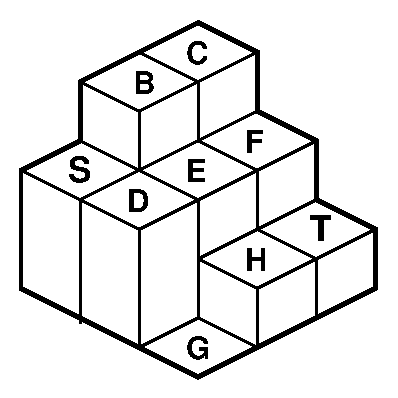
\psfig{file=img/exp_motion.eps,width=5cm}}
\caption{\label{exp_motion}Example of a 3D terrain grid}
\end{figure}

If the cells are of equal elevation, the movement almost always
succeeds, e.g. moving from cell $B$ to cell $C$ in
Figure~\ref{exp_motion}. If the source cell of the motion is lower
than the target cell, then the motion succeeds with low
probability. Furthermore, in this case, a non-zero probability exists
that the direction of motion will be altered. E.g. moving from $H$ to
$E$ is unlikely to succeed, and the agent may end up in $D$, $F$ or
even $G$. If the motion is directed to lower the elevation, it is most
likely will succeed, but also has certain probability to move further
than intended. E.g. moving from $B$ to $E$ is likely to succeed, but
the agent may end up in $H$ or $G$.

Finding an optimal path of motion from $S$ to $T$ and back is,
therefore, becomes non-trivial. Still, if the probabilities of
different transitions are given, the policy iteration algorithm can
easily solve the problem. However, the time it takes the algorithm to
converge to an optimal policy may vary depending on how prominent are
the features of the terrain. Therefore it would be reasonable to
assume that scaling the terrain (and modifying transition
probabilities accordingly) during the initial iterations of learning
will result in faster convergence to the optimal solution. Our
experiments are directed to verify this proposition using our TOP-PI formalism.

{\Large TODO\\ -- CONTINUE WITH REAL DETAILS HERE}

\section{Conclusions and Future Work}\label{sec: future work}

In this paper we have introduced a novel interaction framework between
a teacher and a learner agents. Unlike previous developments in this
area, in our framework the teacher influences the learner indirectly by
modifying the environment away from some normative, passive
dynamics. 

Although in this paper we provide an example based on a learner
executing the policy iteration (PI) algorithm, this limitation is not
a part of our Teacher Optimisation Problem (TOP) framework. Rather it
is a particular instantiation of its principles for the PI
algorithm. As part of our ongoing research we will investigate the
instantiations of TOP with other learning algorithms, particularly
those capable of knowledge transfer~\cite{taylor_stone_2009,taylor_PhD_2008}.

The cost and the effectiveness of the teaching process in TOP can
be measured simultaneously via the Kullback-Leibler divergence rate
(KLR). Specifically, by measuring the KLR between two state-action
processes engendered by the learner's action policy and the
environment dynamics set by the teacher. The detailed choice of the
two processes depends on the interpretation of this cost. One such
interpretation, as the effort it takes to sustain the teaching process
at any given time, is adopted in this paper. As a result the cost is
the KLR between the current policy-environment combination and the
combination of the reference policy with the passive
dynamics. However, in our future work we intend to explore a different
interpretation -- the total effort invested into the teaching
process. In this case the KLR will be between two consecutive
policy-environment combinations plus some final cost expressed by the
KLR between the final policy-environment pair and the combination of
the reference policy with the passive environment dynamics. 


\bibliographystyle{plain}
\bibliography{teacher_em}

%\begin{figure*}[ht]
%{\center 
%\subfigure[Passive dynamics]{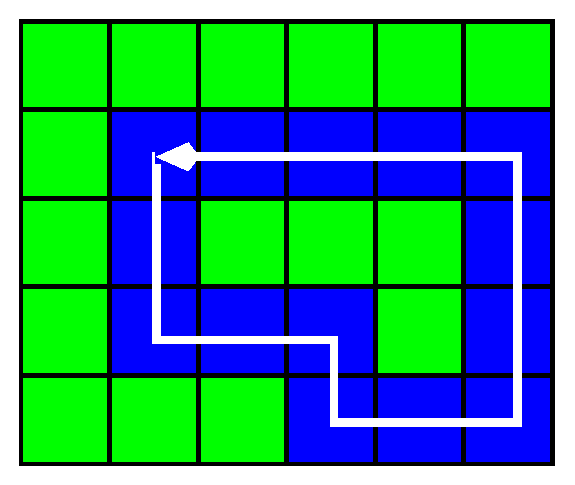
\psfig{file=img/race_track_flat.eps,width=5cm}}
%\subfigure[Augmented dynamics]{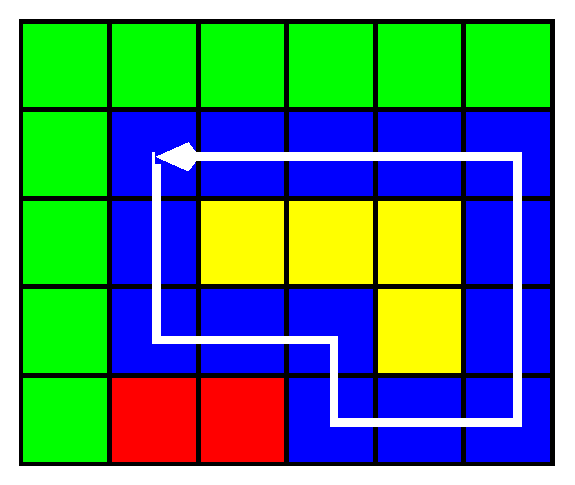
\psfig{file=img/race_track.eps,width=5cm}}\\}
%\caption{\label{race_path}Unmodified (passive) and augmented environment dynamics for race path finding (colours naturally encode traversability of the cell)}
%\end{figure*}

\end{document}
